\documentclass[12pt,oneside]{exam}

% This package simply sets the margins to be 1 inch.
\usepackage[margin=1in]{geometry}

% These packages include nice commands from AMS-LaTeX
\usepackage{amssymb,amsmath,amsthm,amsfonts,latexsym,verbatim,xspace,setspace}
\usepackage{hyperref}
\usepackage{graphicx}

% Make the space between lines slightly more
% generous than normal single spacing, but compensate
% so that the spacing between rows of matrices still
% looks normal.  Note that 1.1=1/.9090909...
\renewcommand{\baselinestretch}{1.1}
\renewcommand{\arraystretch}{.91}

% Define environments for exercises.
\newenvironment{exercise}[1]{\vspace{.1in}\noindent\textbf{Problem #1 \hspace{.05em}}}{}
\newenvironment{newsolution}{\vspace{.1in}\noindent\textbf{Solution: \hspace{.05em}}}{}

% define shortcut commands for commonly used symbols
\newcommand{\R}{\mathbb{R}}
\newcommand{\C}{\mathbb{C}}
\newcommand{\Z}{\mathbb{Z}}
\newcommand{\Q}{\mathbb{Q}}
\newcommand{\N}{\mathbb{N}}
\newcommand{\calP}{\mathcal{P}}
\DeclareMathOperator{\sech}{sech}
\DeclareMathOperator{\csch}{csch}
\DeclareMathOperator{\vsspan}{span}

\newcommand{\func}[3]{{#1} : {#2} \longrightarrow {#3}}

\title{Math 514 - Summer II 2020: Long Quiz 3}

%%%%%%%%%%%%%%%%%%%%%%%%%%%%%%%%%%%%%%%%%%

\begin{document}

\begin{flushright}
\sc MAT 514 - Summer II 2020\\
July 30, 2020
\end{flushright}
\bigskip
 
\begin{center}
\textsf{Solutions to Long Quiz 3} 
\end{center}

%%%%%%%%%%%%%%%%%%%%%%%%%%%%%%%%%%%%%%%%
The objective of this quiz is to use methods of complex integration to solve a real integral, 
\begin{equation*}
\int_{0}^{2\pi} \frac{1}{2+\sin(\phi)}\, d\phi.
\end{equation*}
The problems below will guide you through the solution. 

\begin{exercise}{1}
By expressing the sine function as a combination of complex exponentials, rewrite the integrand as a function of $e^{i\phi}$. 
\end{exercise}

\vspace{0.5cm}

\noindent \textbf{Solution:} By means of the expression 
\begin{equation*}
\sin(\phi) = \frac{e^{i\phi}-e^{-i\phi}}{2i},
\end{equation*}
we may rewrite the integrand in terms of complex exponentials as
\begin{align*}
\frac{1}{2+\sin(\phi)}	& = \frac{1}{2+\frac{e^{i\phi}-e^{-i\phi}}{2i}} \\
& = \frac{2i}{4i+e^{i\phi}-e^{-i\phi}}.
\end{align*}

\vspace{1cm}

\begin{exercise}{2}
Use the substitution $z=e^{i\phi}$ to turn the real-valued integral into a line integral of a rational function in the complex variable $z$. Your answer should take the form
\begin{equation*}
\int_{C[0,1]} \frac{A}{p(z)} \, dz,
\end{equation*}
where $A$ is a constant and $p(z)$ is a quadratic polynomial on $z$.
\end{exercise}

\vspace{0.5cm}

\noindent \textbf{Solution:} Using the suggested substitution, as well as the relation $dz = ie^{i\phi}d\phi$, or equivalently $d\phi = \frac{1}{iz}dz$, we find that the integral may be written as 
\begin{equation*}
\int_{C[0,1]} \left(\frac{2i}{4i +z -\frac{1}{z}} \right)\left( \frac{1}{iz}\right) \, dz = \int_{C[0,1]} \frac{2}{z^2+4iz-1}\, dz.
\end{equation*}

\vspace{1cm}

\begin{exercise}{3}
Factor the polynomial $p(z)$ found in problem 2. Write the integrand from problem 2 as a sum of partial fractions whose denominators have degree one. 
\end{exercise}

\vspace{0.5cm}

\noindent \textbf{Solution:} Using the quadratic formula, we may factor the denominator from problem 2 as 
\begin{equation*}
z^2+4iz-1 = (z+i(2+\sqrt{3}))(z-i(\sqrt{3}-2))
\end{equation*}
A partial fractions decomposition of the integrand in problem 2 takes the form
\begin{equation*}
\frac{2}{z^2+4iz-1} = \frac{A}{z+i(2+\sqrt{3})} + \frac{B}{z-i(\sqrt{3}-2)},
\end{equation*}
where $A$ and $B$ are complex constants satisfying the following system, 
\begin{align*}
A+ B & = 0,\\
(2-\sqrt{3})iA + (2+\sqrt{3})iB & = 2.
\end{align*}
A solution to this system may be easily found by elimination, $A=\frac{i\sqrt{3}}{3}$, $B=-\frac{i\sqrt{3}}{3}$, thus
\begin{equation*}
\frac{2}{z^2+4iz-1} = \frac{i\sqrt{3}}{3z+3i(2+\sqrt{3})} - \frac{i\sqrt{3}}{3z-3i(\sqrt{3}-2)}.
\end{equation*}

\vspace{1cm}

\begin{exercise}{4}
Use Cauchy's Theorem and Cauchy's integral formula to solve the integral 
\begin{equation*}
\int_{0}^{2\pi} \frac{1}{2+\sin(\phi)}\, d\phi.
\end{equation*}
via the method developed in problems 1 through 3. 
\end{exercise}

\vspace{0.5cm}

\noindent \textbf{Solution:} Below is a plot of the two roots of the polynomial $p(z)$ in the complex plane, as well as the path of integration. 
\begin{center}
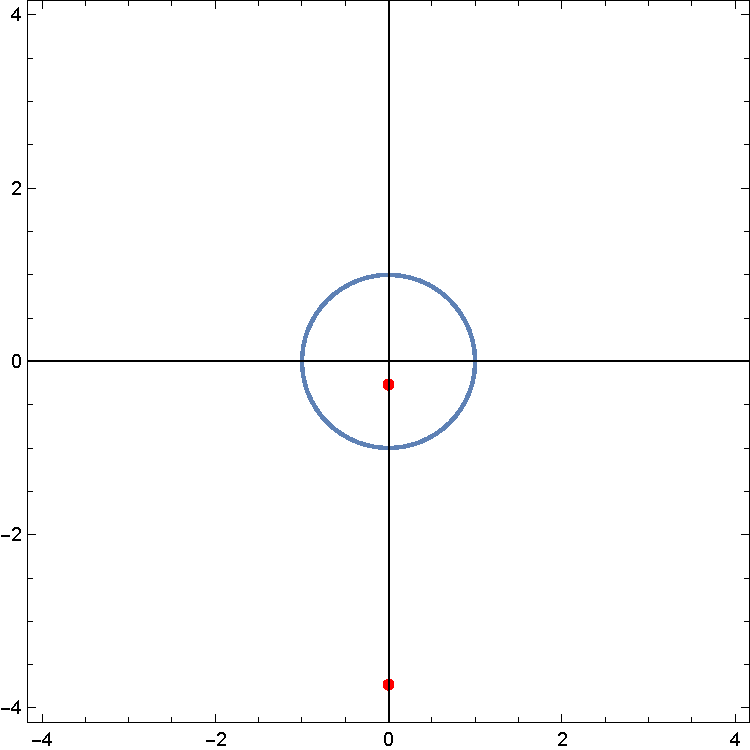
\includegraphics[scale=0.4]{p3.pdf}
\end{center}
We see that one of the roots is contained in the disk bounded by the domain of integration, namely $(\sqrt{3}-2)i$, while the other root $-(2+\sqrt{3})i$, is located outside the disk. We may, therefore, simplify one of the integrals of the partial fractions decomposition by means of Cauchy's Theorem, 
\begin{equation*}
\int_{C[0,1]} \frac{i\sqrt{3}}{3z+3i(2+\sqrt{3})}\, dz = 0.
\end{equation*}
The second component in the partial fractions decomposition is not amenable to this trick. We need to use a homotopy argument and Cauchy's integral formula. Using a homotopy of translations, we may change the path of integration, 
\begin{equation*}
\int_{C[0,1]} \frac{i\sqrt{3}}{3z-3i(\sqrt{3}-2)}\, dz = \int_{C[(\sqrt{3}-2)i,1]} \frac{\frac{i\sqrt{3}}{3}}{z-i(\sqrt{3}-2)}\, dz
\end{equation*}
The value of the latter integral is
\begin{equation*}
\int_{C[(\sqrt{3}-2)i,1]} \frac{\frac{i\sqrt{3}}{3}}{z-i(\sqrt{3}-2)}\, dz = 2\pi i \left(\frac{i\sqrt{3}}{3}\right) = -\frac{2\pi \sqrt{3}}{3}
\end{equation*}
 according to Cauchy's Integral Formula. In summary,
 \begin{align*}
\int_{0}^{2\pi} \frac{1}{2+\sin(\phi)}\, d\phi & = \int_{C[0,1]} \frac{i\sqrt{3}}{3z-3i(\sqrt{3}-2)}\, dz - \int_{C[(\sqrt{3}-2)i,1]} \frac{\frac{i\sqrt{3}}{3}}{z-i(\sqrt{3}-2)}\, dz \\
& = \frac{2\pi \sqrt{3}}{3}.
 \end{align*}
\end{document}

